\section{Current method of ULTRACAM data reduction}

Tom Marsh at the University of Warwick has developed a set of software tools that allow the observer to reduce the data for ULTRACAM. For the rest of this document we will refer to this pipeline as the \emph{traditional} pipeline and the new pipeline created in this project as the \emph{automated} pipeline. 

It is possible to run the traditional pipeline at the telescope during the observation. This allows observers to review the data in 'real-time'. This serves as a `preview' for the observer and allows adjustments to be made during the run. After the run, the raw data is copied to the archive and this can be used for reductions later. This can happen the following day, or much later when the observer has returned from the telescope site. This data archive can be `re-reduced' at any time as all of the raw data is stored in the archive. 

The current data reduction process for ULTRACAM is designed to produce three colour light curves from the raw image data. The pipeline consists of the following stages:
\begin{enumerate}
	\item Producing \emph{bias} frames that are used the calibrate the CCD detector's thermal noise characteristics. 
	\item Producing \emph{flat-fields} to calibrate the pixel sensitivity of each of the 3 CCD detectors. These flat-fields are subtracted from the image data during the reduction process.
	\item Defining \emph{apertures} for the objects of interest in the run. This step involves manually choosing the objects of interest in the frames and defining the aperture sizes and positions for each object. Apertures are independently set for each channel (r, g, b). 
	\item Running the \emph{reduction} software. The reduction code uses the apertures defined in the previous step and measures the flux of each object in each colour. The software is able to track changes in the object's size and shape due to changes in the point spread function (PSF) by scaling the virtual aperture. It is also able to track small deviations in the positions of the objects. 
\end{enumerate} 
Although this process is not particularly cumbersome, it \emph{does} include some manual steps and it does not scale well when there are a large number of runs to be processed or if there are many target objects in a run. For example, the run shown in Fig. \ref{fig:KOI-824} contains more than 1000 objects. Manually defining apertures for each of these objects in each channel is not really practical. An automated method enables data reduction for all of the objects captured in each run without the need for manual intervention. 

\subsection{Aperture selection}

\begin{figure}[!h]
\centering
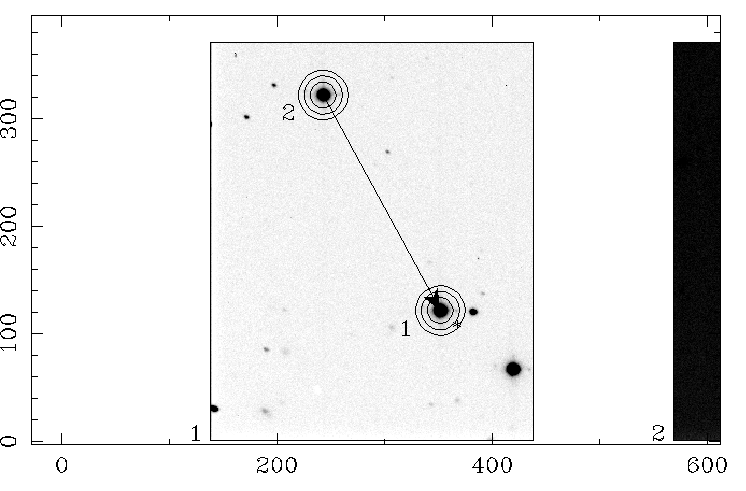
\includegraphics[width=80mm]{images/setaper.png}
\caption{Defining the apertures for the reduction using the \emph{traditional} pipeline. Note that the two apertures can be linked. This instructs the pipeline to maintain the pixel separation of the apertures even if there is a small amount of movement from frame to frame. This is useful if our target object is likely to alter in brightness during the run. }
\label{fig:nnsercomparisontom}
\end{figure}


\subsection{Flat fields and biases}

\subsection{Photometric calibration}

\section{Automating the pipeline}

The outcome of this MSc project is a system that is able to process the raw image data from ULTRACAM and, without any manual intervention, produce a set of light curves for all of the objects in that data. It produces a set of web pages that can be viewed from anywhere with an Internet connection. 

\subsection{Motivation for automating the pipeline}
ULTRACAM has recorded a large amount of photometric data at some of the world's best sites and largest telescopes. Since the CCD captures more objects than the observer is strictly interested in, there is a good chance that some objects of astronomical interest have been captured by ULTRACAM, but not been noticed or analysed during the reduction process. By automating the reduction pipeline we can produce photometry, in other words, 'light curves' for \emph{all} of the objects captured by ULTRACAM and then search through the archive to find new objects of interest. 

An automated pipeline can be run on the data immediately after the run is complete, allowing observers at the telescope to review their results during the course of their observing run. It will also allow collaborators who are not physically at the observatory to browse the data as it is coming in. This enables a strong collaboration with onsite and offsite teams during a run. 

\subsection{Algorithm of the automated pipeline} 

\subsubsection{Key stages for automation}
The stages of the reduction process are as follows:
\begin{enumerate}
	\item Stage 1: Extract all of the 'detectable' objects in all of the frames. 
	\begin{enumerate}
		\item Read the raw image file, containing all frames for a particular run.
		\item Initialise an empty list of objects
		\item For each frame in the run
		\begin{enumerate}
			\item For each colour channel in the frame
			\item Extract each window from the frame
			\item Send the window bitmap data to the SExtractor software
			\item Allow SExtractor to process the data and produce a catalog of all sources, with their positions and flux measurements
			\item Read the results of the source extraction process, including pixel position and flux measurements for each object
			\item For each object returned
			\begin{enumerate} 
				\item Try to match this object with one already in the list, based on nearest distance.
				\item If the object is not already in a list, add this object to the list as a \emph{new} object.
			\end{enumerate}
		\end{enumerate}
		\item Store the list of objects for each of the three channels.
	\end{enumerate}
	\item Stage 2: Filter this list, removing objects that are likely to be artifacts. This is done by looking for objects that do not persist across more than a pre-defined percentage of frames; and objects that have a size approximately equal to one pixel. 
	\item Stage 3: Produce catalogs of the objects ordered by 'brightness' as measured by the average flux. Pass these catalogs to the Astrometry.net library to resolve the WCS solution for the fields. Perform this tasks separately for each of the three channels (r, g, b). Since each channel has a very slightly different view of the field and different distortions in the image, the WCS solutions will differ by a small amount.
	\item Stage 4: Using the WCS solutions, merge the three catalogs to 'cross-identify' each object across the three channels. This may seem to be a trivial step for many ULTRACAM runs because the differences in the fields from channel to channel are minor, however in crowded fields such as the one shown in Fig. \ref{fig:KOI-824} simply matching objects based on their pixel coordinates is not enough to disambiguate them.
	\item Stage 5: Produce deep images for each channel and export to a web-viewable format, such as PNG. 
	\item Stage 6: Create .json data files and HTML files to enable them to be loaded into a web-browser.
	\item Stage 7: Publish this 'web-enabled' data to a web site that is accessible outside of the university network.  
		
\end{enumerate}

\begin{figure}[!h]
	\centering
	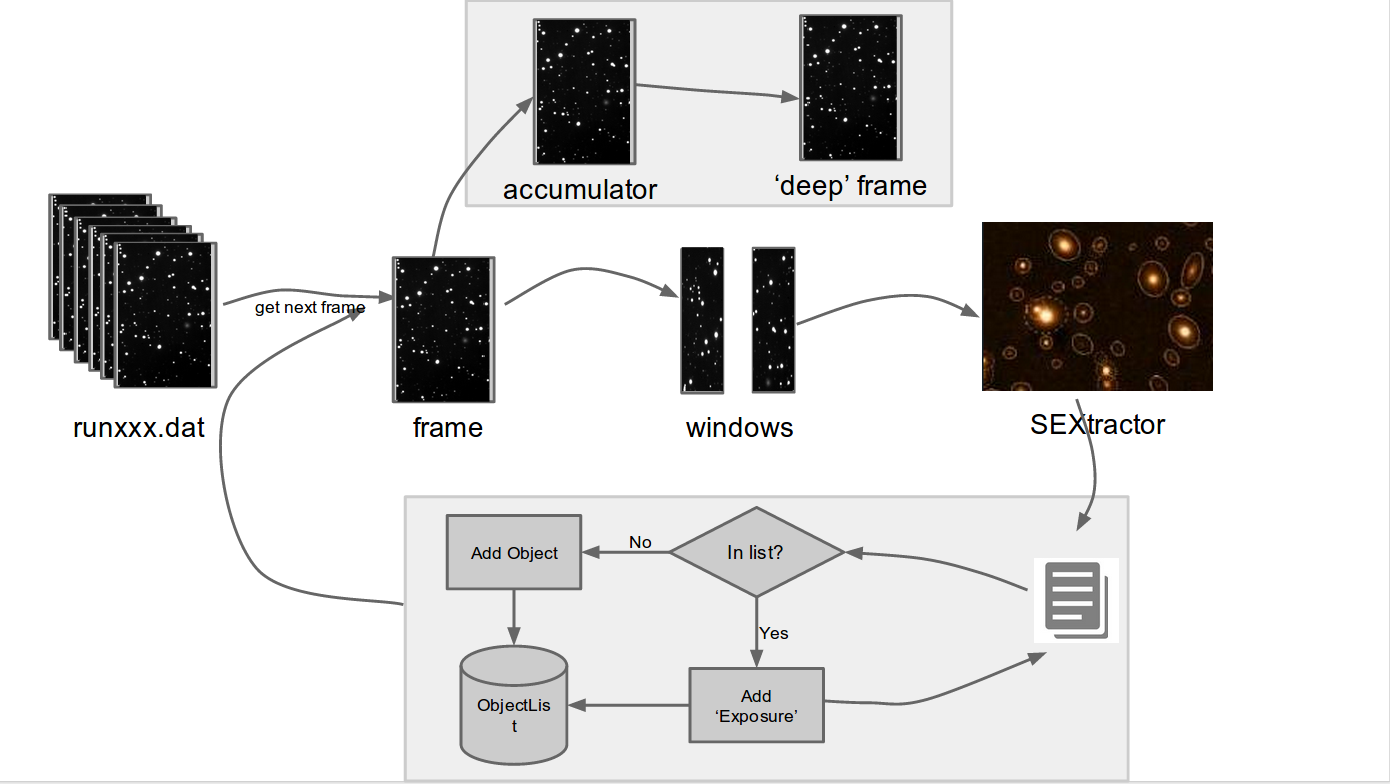
\includegraphics[width=130mm]{images/flowchart.png}
	\caption{Schematic of Stage 1 of the pipeline.}
	\label{flowchart}
\end{figure}


\begin{figure}[!h]
	\centering
	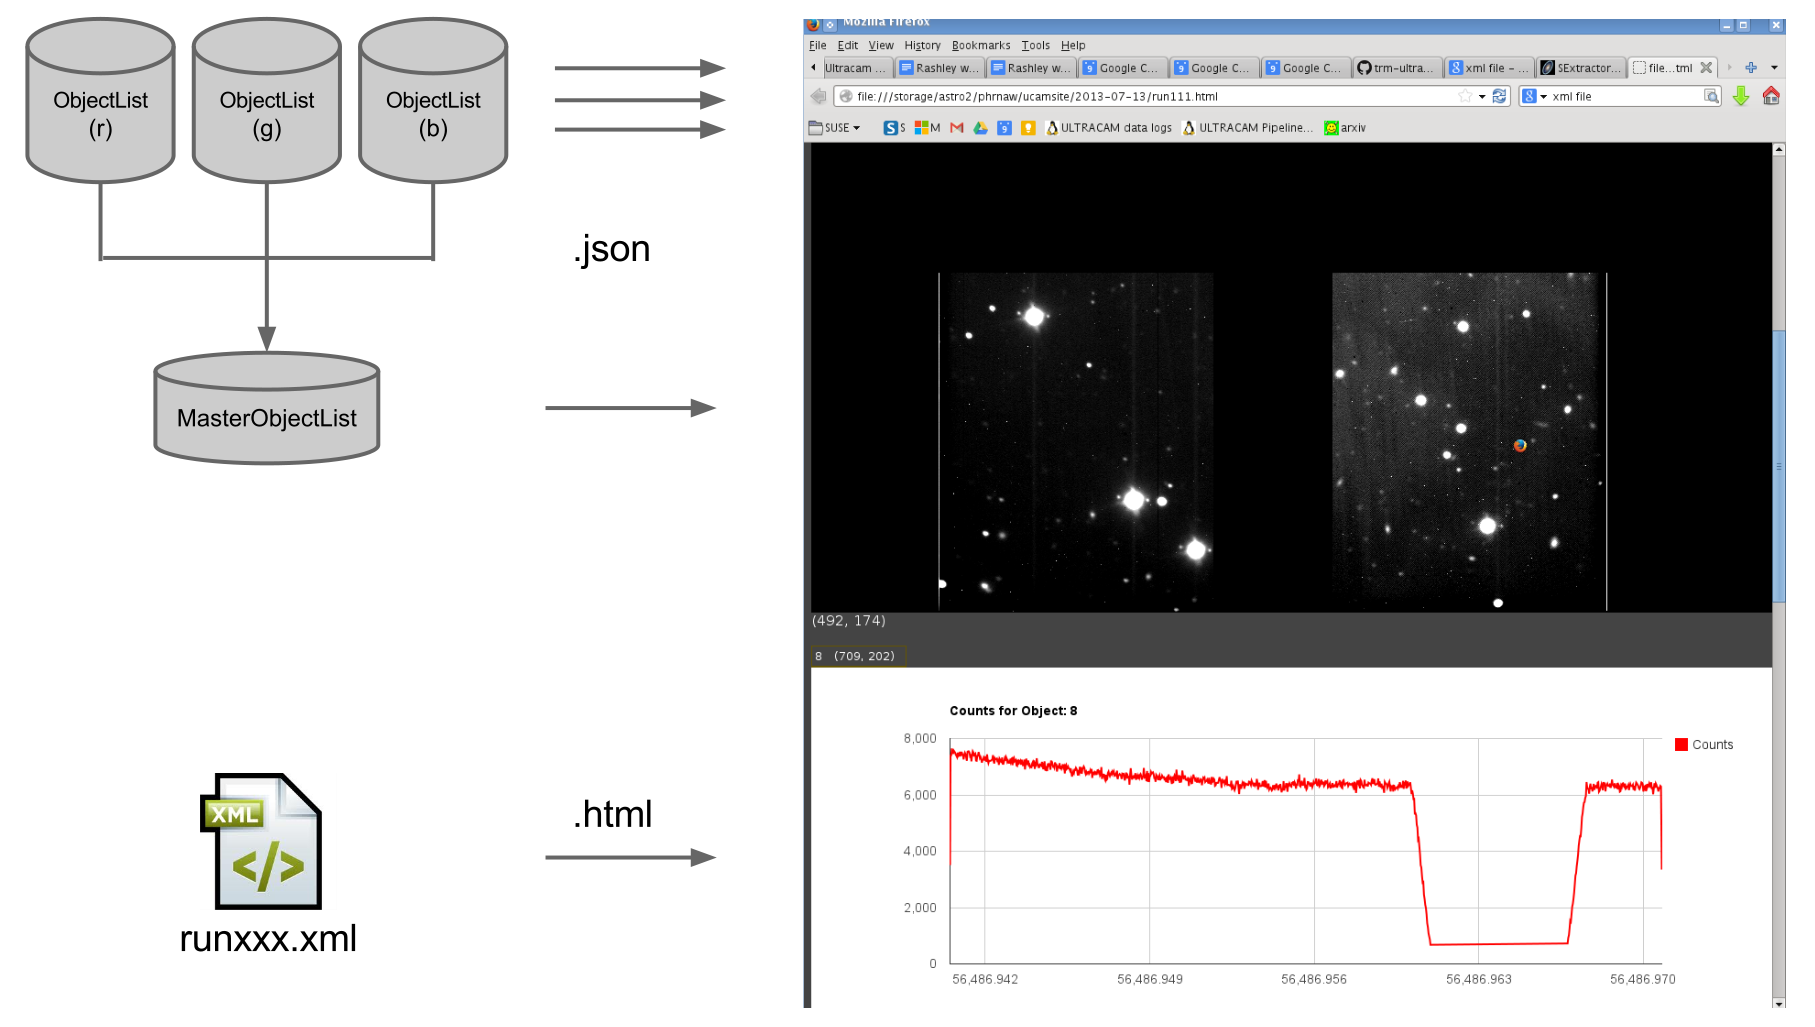
\includegraphics[width=130mm]{images/webpublish.png}
	\caption{Schematic of Stage 6 and 7 of the pipeline.}
	\label{webpublish}
\end{figure}

\subsubsection{Source extraction}
A popular software tool used for source extraction is SExtractor \cite{bertin}. SExtractor is able to process an image field and produce a catalog of sources in that field along with a measurement of the flux count of each object. The flux count is calculated after making efforts to account for the background in the field and then fitting a profile to the object. 

To follow: More info on how SExtractor performs the sky substraction, aperture fitting and flux measurement. Much of it pulled from the SExtractor manual. 

\subsection{Object matching}

Analysis of the techniques used for object matching. First pass using pixel location and independent on each channel. 

Second pass to identify the same object on different channels using pixel coordinates, as well as astrometric solutions (if available). 

\subsection{WCS solutions}

Discussion of using the Astrometry.net package. 

After some ad-hoc tests using \emph{SCAMP \cite{scamp}} and \emph{Astrometry.net \cite{astrometry}} it seemed that the Astrometry.net software was more reliable at finding good WCS solutions to the fields. The software was downloaded to a local machine (including the extensive index files) and compiled. At the moment, this is now part of the pipeline but it does not consistently find WCS solutions for all of the fields. 

There are several challenges to finding a WCS solution for the fields.  These are:
\begin{itemize}
	\item \emph{Lack of pointing data}: The Ultracam system does not integrate with the pointing software of any of the telescopes and does not get pointing information automatically. We rely on the observer to enter a name of the candidate object for each run and then, when the data is archived, a \emph{SIMBAD} lookup is used. This gives us a world coordinate that is somewhere in the field, but it is not known which object (or pixel location) this applies to.  
	\item \emph{Field rotation}: Since the Ultracam can be rotated about the optical axis to allow for optimal alignment of the objects, this means that the field of view can be at any arbitrary rotation giving an extra degree of freedom to the matching task. 
	\item \emph{Windows}: Many ULTRACAM runs are configured to use only portions of the CCD area. You can see an example of this in Fig.  \ref{fig:V713Cep}. This means that there is an incomplete view of the sky for that field. When trying to match to existing indexes, there could be important, bright objects that are in the index file, but do not appear in the Ultracam field due to the masking caused by the windows.
	\item \emph{Sparse fields}: On uncrowded fields, we might only have 4-5 objects that can be used for field identification. 
	\item \emph{Very small windows}: Some runs, particularly ones in high cadence mode, use very small windows (eg 172x156 pixels) in order to decrease readout time. This means that the Ultracam images might only contain two objects or so. This makes matching to a reference catalog impossible. 
	\item \emph{Choice of reference index by colour}: The Astrometry.net software uses 2MASS and Tycho-2 reference catalogs by default. These are based on infra-red and V magnitudes. This means that the blue channel (which is often using the SDSS u filter) might not match the reference indexes. Indeed, current tests often end with a match in red, a match in green and no match in blue. 
\end{itemize}

\subsection{Web publishing}

Discussion of the choices made in publishing to the web. Particularly the pros and cons of doing all of the web interaction in the client and also the choice of JSON as the data transport mechanism. 

The core `visible product' of the project is a website that allows a user to browse all of the data in the ULTRACAM archive. The key features of this website are:

\begin{itemize}
	\item A catalog of runs organised by calendar date, containing \emph{thumbnail images} of the fields.
	\item For each run, a web page that shows the user:
	\begin{itemize}
		\item the \emph{deep images} of the field in each of the three channels (r, g, b).
		\item the \emph{light-curves} of each object as the user clicks on the object with the mouse. 
		\item the sky coordinates of each object and the mouse position, provided that a correct astrometric solution has been found for the run. 
		\item the light curve for the object that is currently being used as the 'comparison' object. 
	\end{itemize}
	\item light-curves should be plotted as absolute measured flux or a \emph{relative flux} compared to some other objects in the field. 
	\item the web page should also allow the user to \emph{export} the data to a standard format.
	
\end{itemize}
See Fig. \ref{browser} for an example of the web-page. 

\begin{figure}[!h]
	\centering
	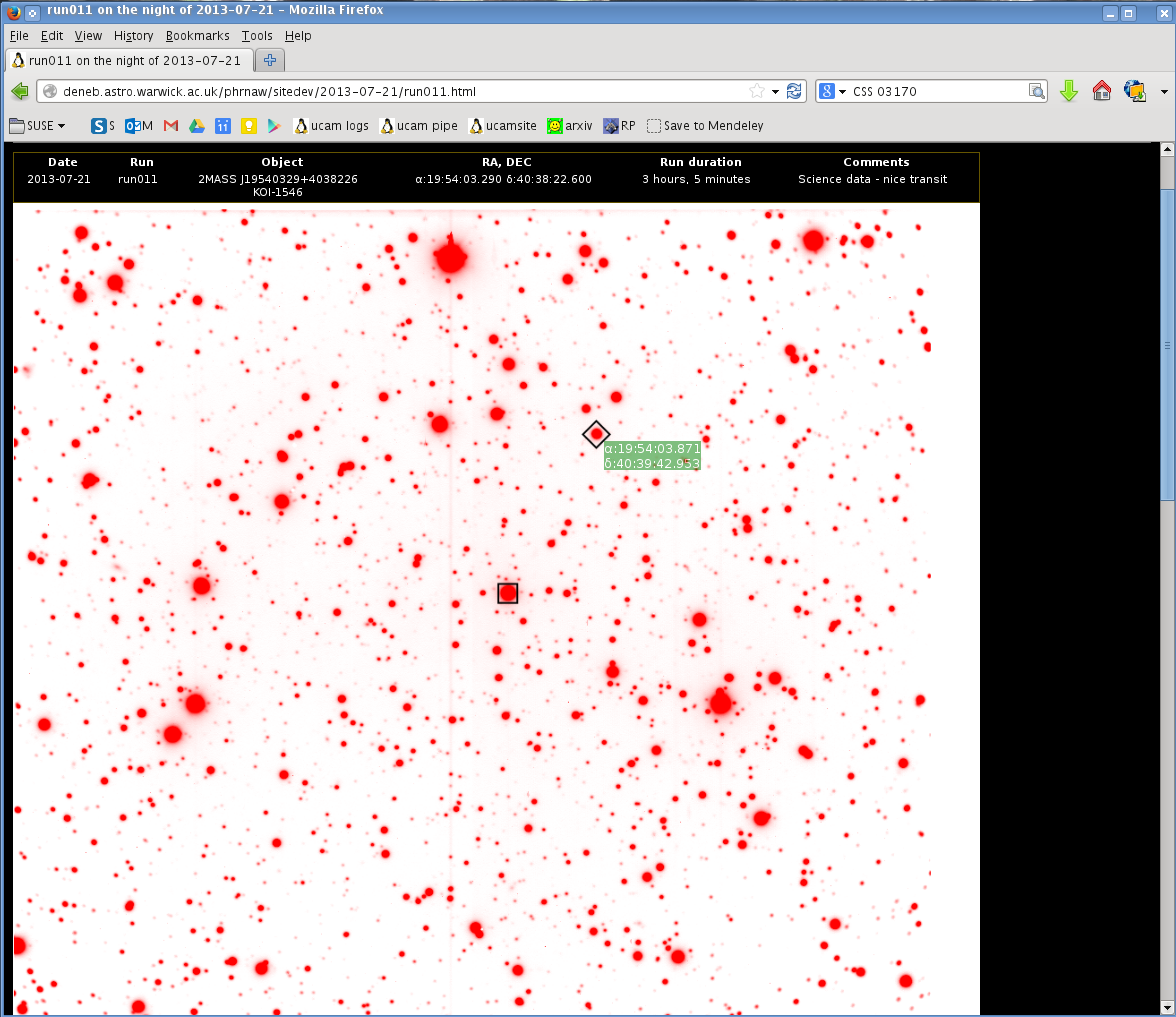
\includegraphics[width=90mm]{images/website1.png}
	\caption{Preview of the webpage.}
	\label{browser}
\end{figure}

